\section{Experimental Evaluation}
\label{sec:evaluation}
We have carried out the attacks on 22 OAuth2.0 providers. They are : 
\begin{itemize}
\item Google
\item Yammer
\item VK
\item Stripe
\item Basecamp
\item Zendesk
\item Box
\item Formstack
\item Github
\item Reddit
\item Yandex
\item Twitch
\item Instagram
\item Foursquare
\item Fitbit
\item Imgur
\item Linkedin
\item Salesforce
\item Strava
\item Dropbox
\item Battle.net
\item Yahoo
\end{itemize}
We present the different results below. 
\subsection{Login CSRF}
Out of the 22 providers examined, 7 were vulnerable to this attack and the rest were found non vulnerable. For the vulnerability, we tested two kinds of scenarios. These scenarios depend on the login form presented to the user as part of the OAuth2.0 flow and another as part of the normal login page that a user might land on when he/she enters the website's login page address in the address bar. This is important because for some of the providers the login form presented to the user during the OAuth flow might be different from the normal login page he/she is usually redirected to. In such a case, the two login forms might not have the protection enabled in both and hence can be exploited. 
\begin{enumerate}[label=(\Alph*)]

\begin{figure}[t]
   		 \centering
   		 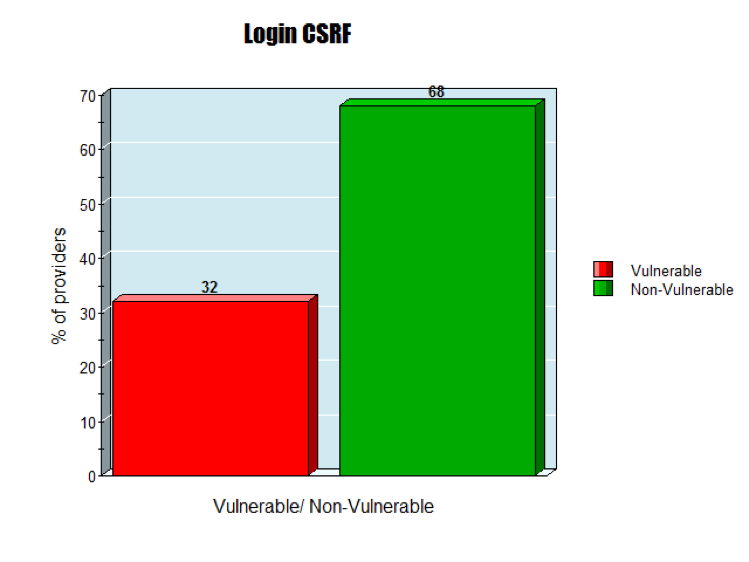
\includegraphics[width=\columnwidth]{figures/loginstats.png}.
   		 \caption{Login CSRF}
   		 \label{fig:logincsrf}
\end{figure}
	
\item \textit{Vulnerable:}
The following were vulnerable to the attack :
	\begin{itemize}
	\item \textbf{Reddit.} An attacker has to just forge a simple form with "user" and "passwd" and submit it to the Reddit login endpoint. Here the user is redirected to the same generic login page and hence only one form is involved.  
	
	\item \textbf{Formstack.} This site involves two login forms as explained above. The form in the OAuth flow is vulnerable to attack as it involves sending only the user email and password. However in the normal login page is not vulnerable because it contains a hidden CSRF token field that is sent along with user email and password form data.  
	
	\item \textbf{Basecamp.} This site is vulnerable in both scenarios. There is an authenticity token being sent as part of the login request but it is not being checked by the provider consequently allowing the attacker to forge a login request.
	
	\item \textbf{Yandex.} This site is vulnerable because it does not contain any kind of a CSRF token and only user credentials are sent as part of the login request. 
	
	\item \textbf{Yammer.} This site is interesting because it needs a organizational email to login. When we tested with our uic.edu email ID it redirected us to the UIC login which did not contain a CSRF token and hence could be exploited to login into Yammer.
	
	\item \textbf{Fitbit.} This site is vulnerable because it does not contain any kind of a CSRF token and only user credentials are sent as part of the login request. 
	
	\begin{figure}[t]
   		 \centering
   		 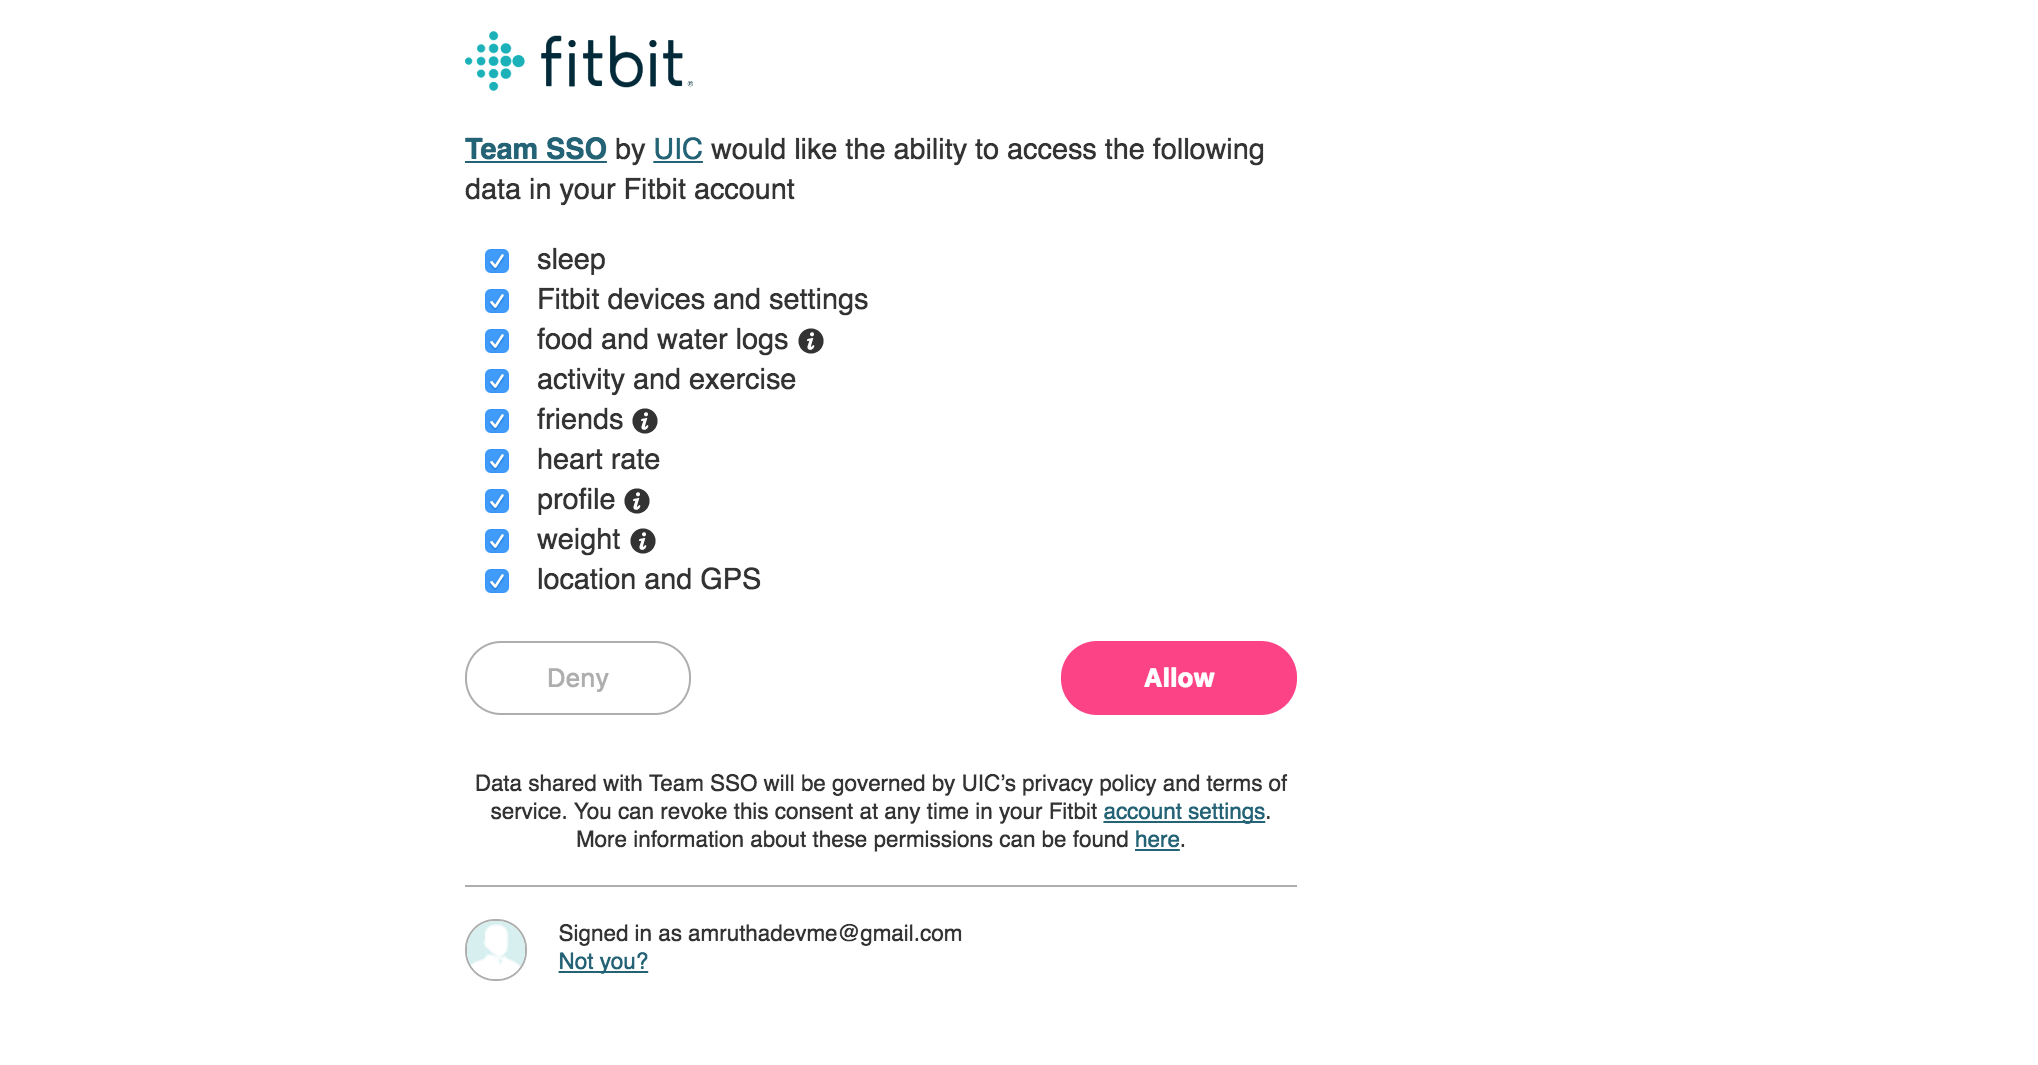
\includegraphics[width=\columnwidth]{figures/vulnerable/fitbit1.png}.
   		 \caption{Login CSRF : Screenshot of Fitbit}
   		 \label{fig:fitbit}
	\end{figure}
	
	\item \textbf{Imgur.} This site is vulnerable because it does not contain any kind of a CSRF token and only user credentials are sent as part of the login request. 
	
	\end{itemize}
\item\textit{Non vulnerable:}
	The rest of the providers were not vulnerable because most of them included some kind of login CSRF token in their forms. VK had three randomly generated values that is sent with every login form submission instead of a CSRF token. Stripe sent a dynamically generated token value in the request but that was not present in the form itself. Salesforce had a two step verification process and sent a code request was sent in a message to your email id whenever a login was attempted. Dropbox and Battlenet had a very complex request JSON that could not have been replicated. 
\end{enumerate}

\textit{Note :} Please see Appendix\ref{sec:appendix} for the screenshots of other providers vulnerable to login CSRF.

\subsection{Redirect URI Mismatch}
We redirected the user-agent to the authorization server, including information identifying itself (a client id), the request (scope - the permissions being requested), and a URL pointing back to the client (here we used a redirect URL that was different from the one we used for registering the application).Ideally, the authorization server should give a redirect URI mismatch error (which we got in most cases) However, there were some providers which did not check for the mismatch and the authorization server authorized the resource owner, and performed authentication such as username/password verification, and confirmation of the action requested. On success, it directed the user-agent back to the client through the provided redirect URL, adding an authorization code to the URL. 
We have registered the application with all the providers with the https://team-sso.appspot.com/<callbackname> and we are trying to redirect the code to an unregistered subdirectory https://team-sso.appspot.com/<callbackname>/test or a different directory https://team-sso.appspot.com/maliciousapp.

\begin{enumerate}[label=(\Alph*)]
\item \textit{Vulnerable :}  A few providers did not check for the redirect URI mismatch. This led them to send the authorization code to another directory or subdirectory of the registered redirect URI. This code could then be exchanged by the attacker for the access token. Using the access token the attacker could make API requests from the user's account and access whatever services he wants from the provider on behalf of the user.
The providers who leaked and token to a subdirectory are :
\begin{itemize}
\item Box
\item Github
\item Formstack
\item Foursquare
\item Imgur
\item Yahoo
\item Strava
\end{itemize}

\begin{figure}[t]
   		 \centering
   		 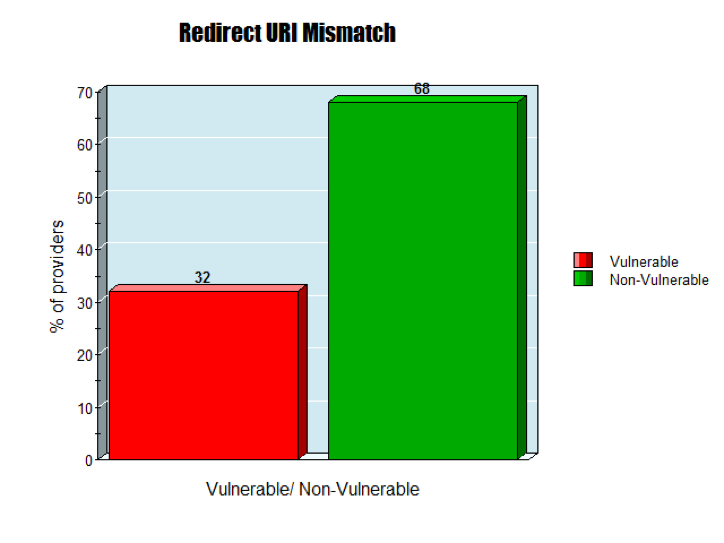
\includegraphics[width=\columnwidth]{figures/redirectstats.png}.
   		 \caption{Redirect URI Mismatch}
   		 \label{fig:statsredirect}
\end{figure}
	
	
Among these the providers who leaked and token to another malicious directory are :
\begin{itemize}
\item Yahoo
\item Strava
\end{itemize}

\begin{figure}[t]
   		 \centering
   		 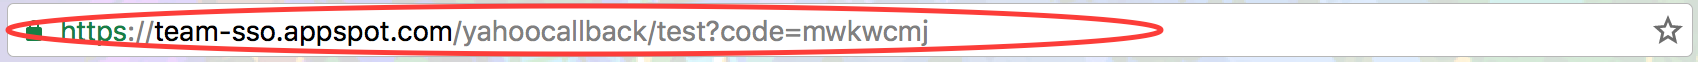
\includegraphics[width=\columnwidth]{figures/yahoo1.png}.
   		 \caption{Redirect URI Mismatch : Yahoo }
   		 \label{fig:yahooredir}
\end{figure}



\item \textit{Non Vulnerable :}  The other providers implemented the check for mismatch of redirect URI and did not leak the code to another URL other than the exact one registered with the provider. They all gave a general redirect URI mismatch error while attempting the attack.

\begin{figure}[t]
   		 \centering
   		 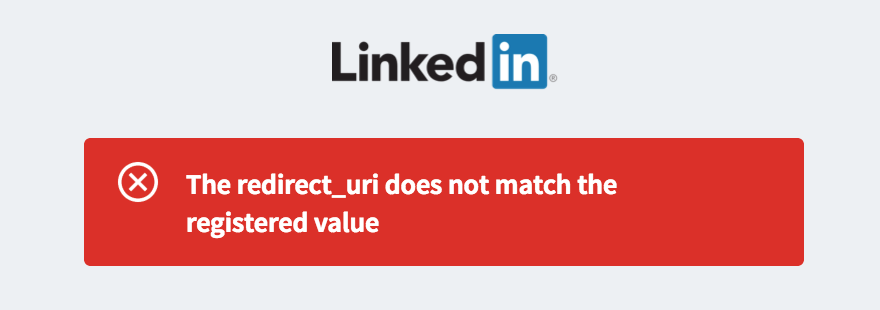
\includegraphics[width=\columnwidth]{figures/linkedin1.png}.
   		 \caption{Redirect URI Mismatch : Linkedin }
   		 \label{fig:linkredir}
\end{figure}


\end{enumerate}
\textit{Note :} Please see Appendix\ref{sec:appendix} for the screenshots of other providers vulnerable to redirect URI mismatch.


\subsection{Cover redirect}The access token which is exchanged for the code should never be requested directly i.e. it should never be a direct part of the request parameters. However, many providers allowed for this to be a valid scenario. We attempted the attack by changing the response type parameter in the request to token instead of code which should ideally be invalid. We were able to get the token in the fragment of the URI which could be accessed by any third party on the page by JavaScript using location.hash and this would give them access to make API calls on behalf of the user to any provider service. This combined with the redirect URI mismatch would be even more dangerous because if the access token is given in the URL for a malicious client it can further be accessed by all the malicious third parties present on their page as well the malicious client itself.

\begin{figure}[t]
   		 \centering
   		 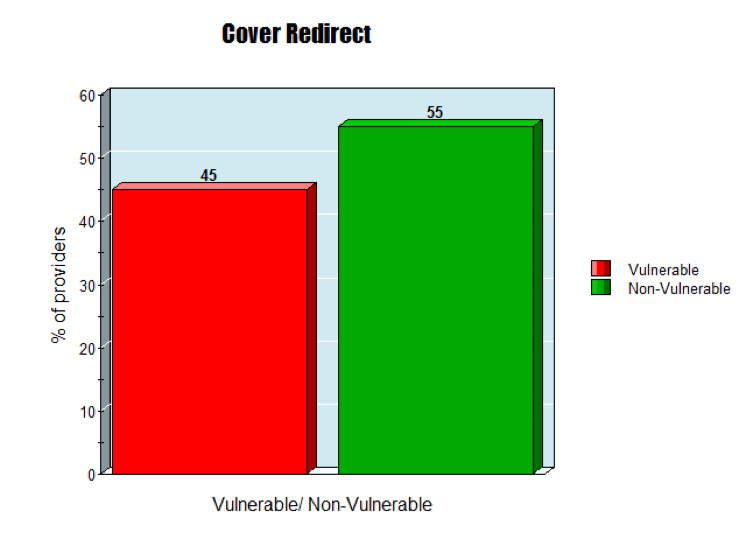
\includegraphics[width=\columnwidth]{figures/coverstats.png}.
   		 \caption{Cover Redirect : Salesforce }
   		 \label{fig:salesredir}
\end{figure}

\begin{enumerate}[label=(\Alph*)]
\item \textit{Vulnerable :} Most providers allowed this scenario for the registered redirect URI at the provider. These providers were :
\begin{itemize}
\item Yammer
\item Yahoo
\item Formstack 
\item VK
\item Yandex
\item Twitch
\item Salesforce
\item Dropbox
\item Imgur
\item Foursquare
\end{itemize}

\begin{figure}[t]
   		 \centering
   		 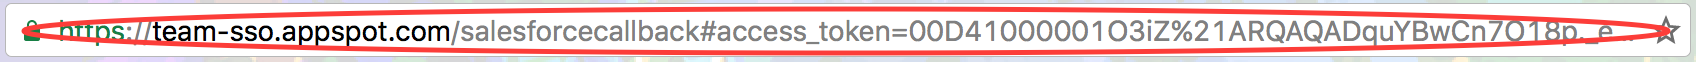
\includegraphics[width=\columnwidth]{figures/salesforce1.png}.
   		 \caption{Cover Redirect : Salesforce }
   		 \label{fig:salesredir}
\end{figure}

Among these some which leaked the token in the URL for even unregistered directories and sub-directories were :
\begin{itemize}
\item Imgur
\item Foursquare
\item Formstack
\item Yahoo
\end{itemize}

\item \textit{Non Vulnerable :} The other providers that were non-vulnerable to this attack gave a common error of bad request which indicated that the response type was invalid and token could not be requested directly. This is the correct implementation which all providers should adopt.

\begin{figure}[t]
   		 \centering
   		 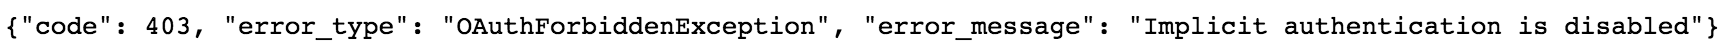
\includegraphics[width=\columnwidth]{figures/instagram.png}.
   		 \caption{Cover Redirect : Instagram }
   		 \label{fig:instaredir}
\end{figure}

\end{enumerate}
\textit{Note :} Please see Appendix\ref{sec:appendix} for the screenshots of other providers vulnerable to cover redirect.

\begin{figure}[t]
   		 \centering
   		 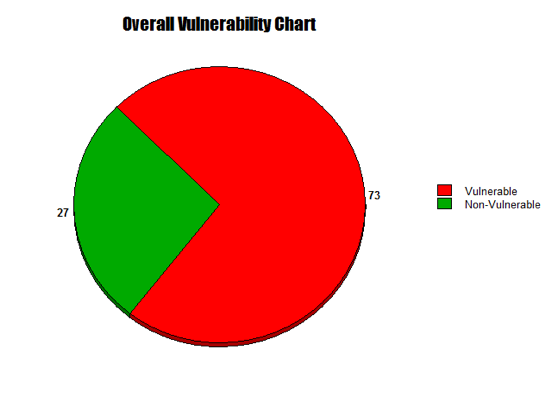
\includegraphics[width=\columnwidth]{figures/overall.png}.
   		 \caption{Overall Vulnerability Chart }
   		 \label{fig:overall}
\end{figure}

In the end, we found that 32 percent of the providers were vulnerable to our redirect URI mismatch and Login CSRF attacks whereas 45 percent were vulnerable to the Cover redirect attack. Overall, 73 percent of the providers were vulnerable to one or the attack and 27 percent were not vulnerable to any.

